\apendice{Documentación de usuario}

\section{Introducción}

En este apéndice se explican los requisitos que debe cumplir el usuario de la aplicación para ejecutarla y utilizarla. Cabe destacar que la aplicación está en inglés por petición del cliente.

\section{Requisitos de usuarios}

Dado que se trata de una aplicación web, lo único que necesita el cliente es tener instalado un navegador web que soporte \textit{Javascript}, \textit{jQuery} y hojas de estilo CSS.

Los navegadores soportados serán:
\begin{itemize}
	\item Google Chrome.
	\item Mozilla Firefox.
	\item Microsoft Edge.
	\item Internet Explorer 9 o superior.
	\item Safari.
	\item Opera.
\end{itemize}

\section{Instalación}

El usuario, en un primer momento, no tendrá que realizar ninguna instalación pues al tratarse de una aplicación web, le bastaría con acceder desde uno de los navegadores ya comentados al siguiente enlace: 

\url{https://www.proyectoubu.nesiweb.com/}

\section{Manual del usuario}

En esta sección se va a explicar al usuario cómo utilizar la aplicación.

Se desglosará la aplicación por módulos que se explicarán por separado:
\begin{itemize}
	\item Login.
	\item Administración de entidades mediante formularios.
	\item Administración de entidades mediante hojas de cálculo.
	\item Restauración de base de datos a su estado inicial de test.
	\item Generación de la simulación.
	\item Ejecución de la simulación.
	
\end{itemize}

\subsection{Login}

En primer lugar, nos llevará a una \href{https://www.proyectoubu.nesiweb.com/users/login}{pantalla de acceso}~\ref{img:login}. Como ya se ha comentado, hay usuarios con distintos roles:
\begin{itemize}
	\item Rol administrador.
	\item Rol participante.
\end{itemize}

Dependiendo del rol que tenga el usuario conectado, las funcionalidades disponibles serán diferentes.

En la ilustración~\ref{img:DashboardAdmin} se puede ver la pantalla principal de un usuario con rol administrador, mientras que la figura~\ref{img:DashboardPart} representa la pantalla principal de un usuario con rol participante.

Un administrador podrá restablecer la base de datos a su estado de test inicial y además cuenta con una administración de usuarios. Un usuario con rol participante solo podrá gestionar su propia información.

\begin{figure}[h]
	\centering
	
\includegraphics[width=1\textwidth]{/anexos/ManualUsuario/Login}
	\caption{Pantalla de acceso a la aplicación.}
	\label{img:login}
\end{figure}

\begin{figure}[h]
	\centering
	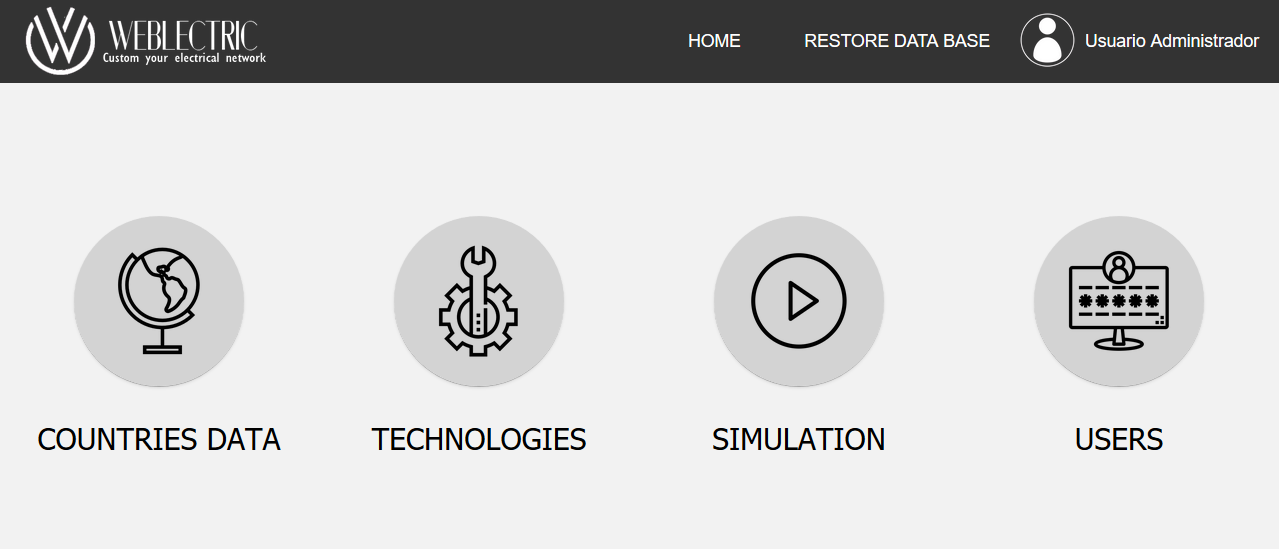
\includegraphics[width=1\textwidth]{/anexos/ManualUsuario/DashboardAdmin}
	\caption{\textit{Dashboard} usuario con rol administrador.}
	\label{img:DashboardAdmin}
\end{figure}

\begin{figure}[h]
	\centering
	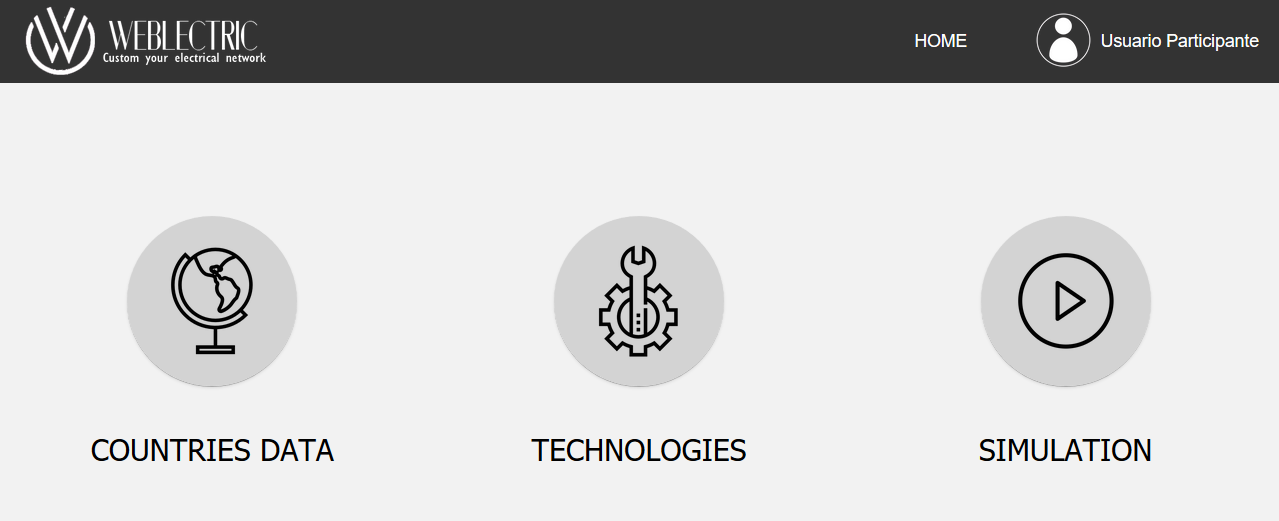
\includegraphics[width=1\textwidth]{/anexos/ManualUsuario/DashboardParticipant}
	\caption{\textit{Dashboard} usuario con rol participante.}
	\label{img:DashboardPart}
\end{figure}

\newpage

\subsection{Administración de entidades mediante formularios}

Esta funcionalidad está presente para los dos tipos de usuarios. 

En la aplicación, son muchas las entidades que se administran a través de formularios. Un ejemplo pueden ser los combustibles.

En la figura~\ref{img:FuelsHome} aparecen listados los combustibles presentes en la aplicación. Además, como se observa en la imagen, se puede dar de alta, modificar o eliminar un elemento. El formulario correspondiente a los combustibles se puede ver en la figura~\ref{img:FuelsForm}.

Para evitar el almacenamiento de datos erróneos en base de datos, es común la presencia de validaciones para los campos que se administran a través de formularios. 

\begin{figure}[h]
	\centering
	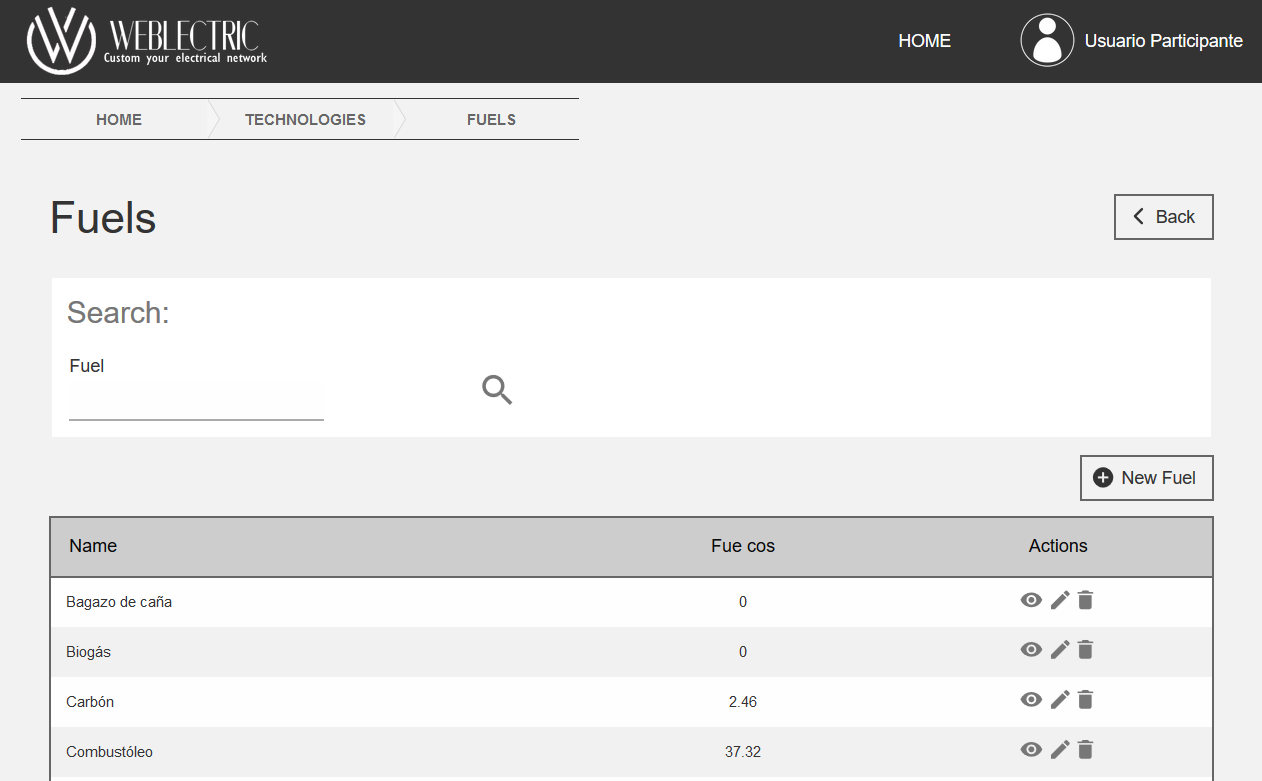
\includegraphics[width=0.9\textwidth]{/anexos/ManualUsuario/FuelsHome}
	\caption{Pantalla principal de los combustibles.}
	\label{img:FuelsHome}
\end{figure}

\begin{figure}[h]
	\centering
	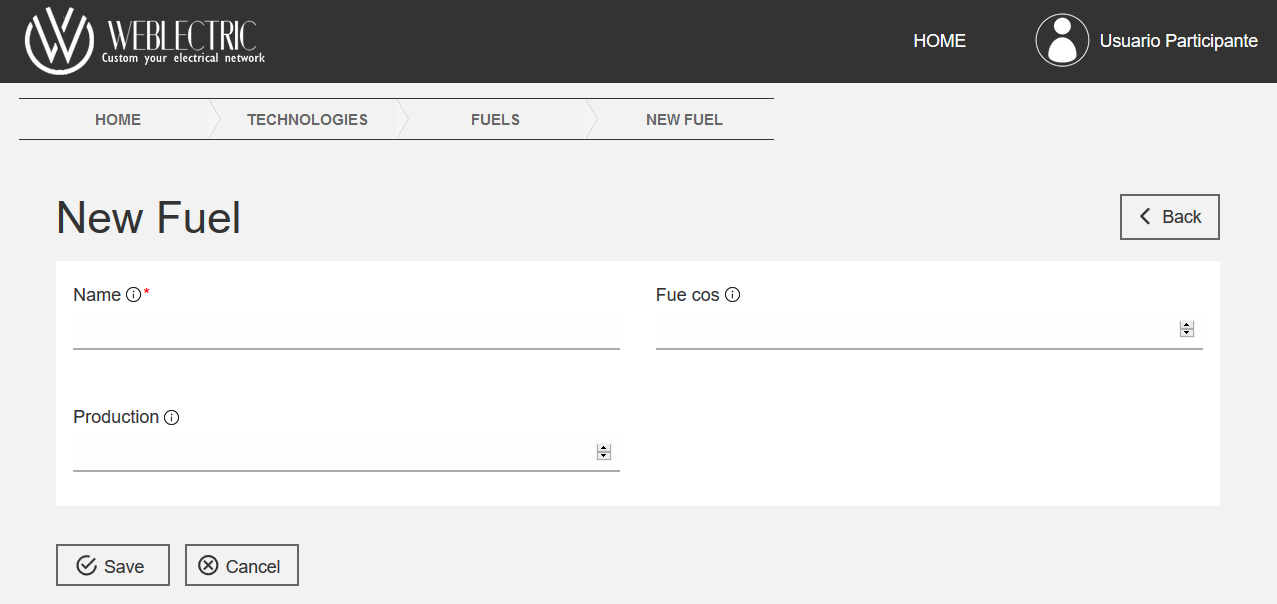
\includegraphics[width=1\textwidth]{/anexos/ManualUsuario/FuelsForm}
	\caption{Formulario para crear o editar un combustible.}
	\label{img:FuelsForm}
\end{figure}

\newpage

\subsection{Administración de entidades mediante hojas de cálculo}

En la aplicación, tenemos tres tablas que se administran mediante hojas de cálculo:
\begin{itemize}
	\item \href{https://www.proyectoubu.nesiweb.com/rangerenewables/technologies}{rangerenewables}: Datos de fuentes renovables en un instante de tiempo concreto.
	\item \href{https://www.proyectoubu.nesiweb.com/rangedemands/home}{rangedemands}: Datos de demanda en un instante de tiempo concreto.
	\item \href{https://www.proyectoubu.nesiweb.com/rangemeteos/home}{rangemeteos}: Datos meteorológicos en un instante de tiempo concreto.
\end{itemize}

Los campos detallados están explicados en el diccionario de datos del anexo ``Especificación de diseño''~\ref{title:DiccionarioDatos}. 
 
En la figura~\ref{img:Rangedemands} se puede ver un ejemplo de lo que es la pantalla principal desde donde se puede descargar la hoja de cálculo con los datos actuales o subir un archivo para actualizar los datos.
 
\begin{figure}[h]
	\centering
	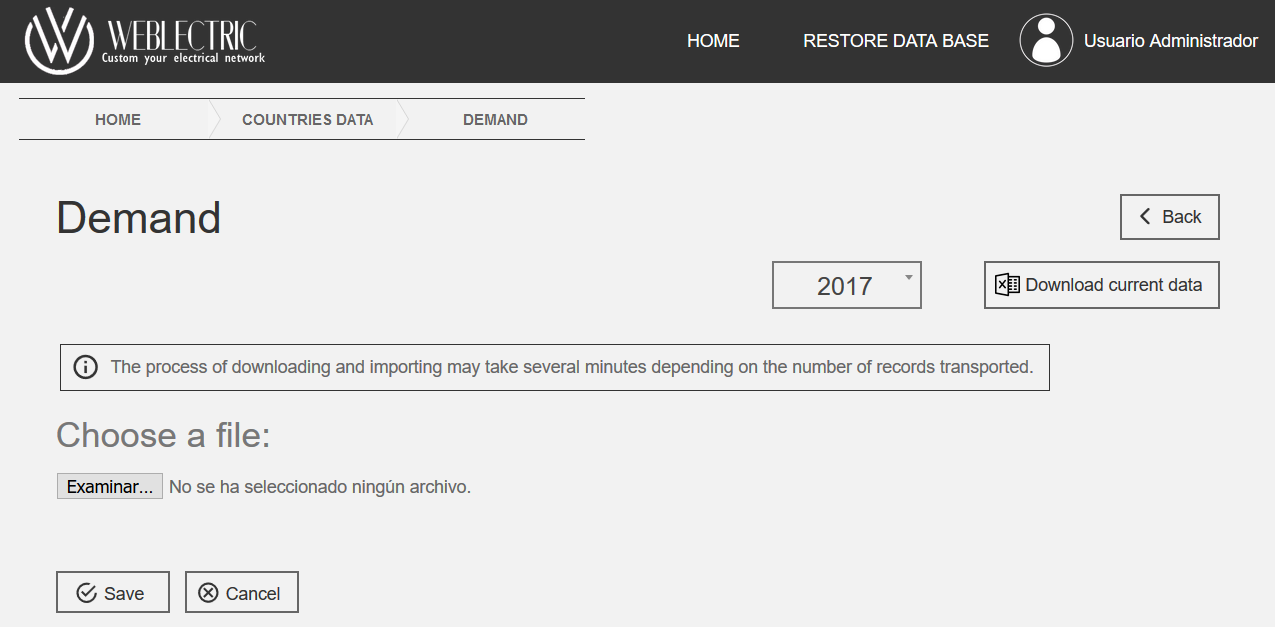
\includegraphics[width=1\textwidth]{/anexos/ManualUsuario/Rangedemands}
	\caption{Página principal de una tabla administrada mediante hojas de cálculo.}
	\label{img:Rangedemands}
\end{figure}

Se puede observar la presencia de un selector con diferentes años. Este desplegable tiene dos funcionalidades:
\begin{itemize}
	\item En la descarga de los datos actuales, se descargarán los datos del año seleccionado.
	\item En la importación de datos, se eliminarán los datos presentes en base de datos para el año seleccionado y se sustituirán por los cargados mediante la hoja de cálculo.
\end{itemize}

La hoja de cálculo a utilizar para esta administración ha de tener un aspecto como el que muestra la figura~\ref{img:RangedemandsExcel}. En las columnas aparece el año, mes, día, hora y después una columna por cada región de transmisión del país y cada fila representa un instante en el tiempo.

\begin{figure}[h]
	\centering
	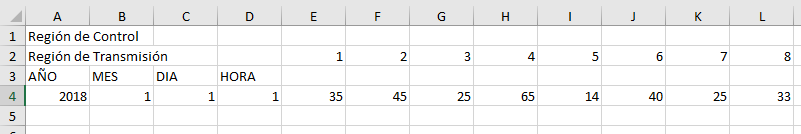
\includegraphics[width=1\textwidth]{/anexos/ManualUsuario/RangedemandsExcel}
	\caption{Ejemplo de hoja de cálculo.}
	\label{img:RangedemandsExcel}
\end{figure}

\newpage

\subsection{Restauración de base de datos a su estado inicial de test}

Como ya se ha comentado, esta funcionalidad está presente para aquellos usuarios con rol administrador. Su desarrollo está enfocado para que el usuario pueda realizar pruebas y mantenimiento sobre la aplicación con la libertad de volver al estado inicial de test si se considera oportuno.

Para ello, en el gestor de bases de datos utilizado, se ha creado una base de datos de respaldo hacia la cual se realiza la consulta cuando se desea restablecer la información. Al usuario de la base de datos se le ha dado privilegios globales para que pueda hacer una consulta sobre cualquier base de datos.

Esta funcionalidad se desempeña a través de un botón situado en la cabecera de la aplicación. En la figura~\ref{img:Restore} se puede observar el mensaje de aviso previo a la restauración de los datos.

\begin{figure}[h]
	\centering
	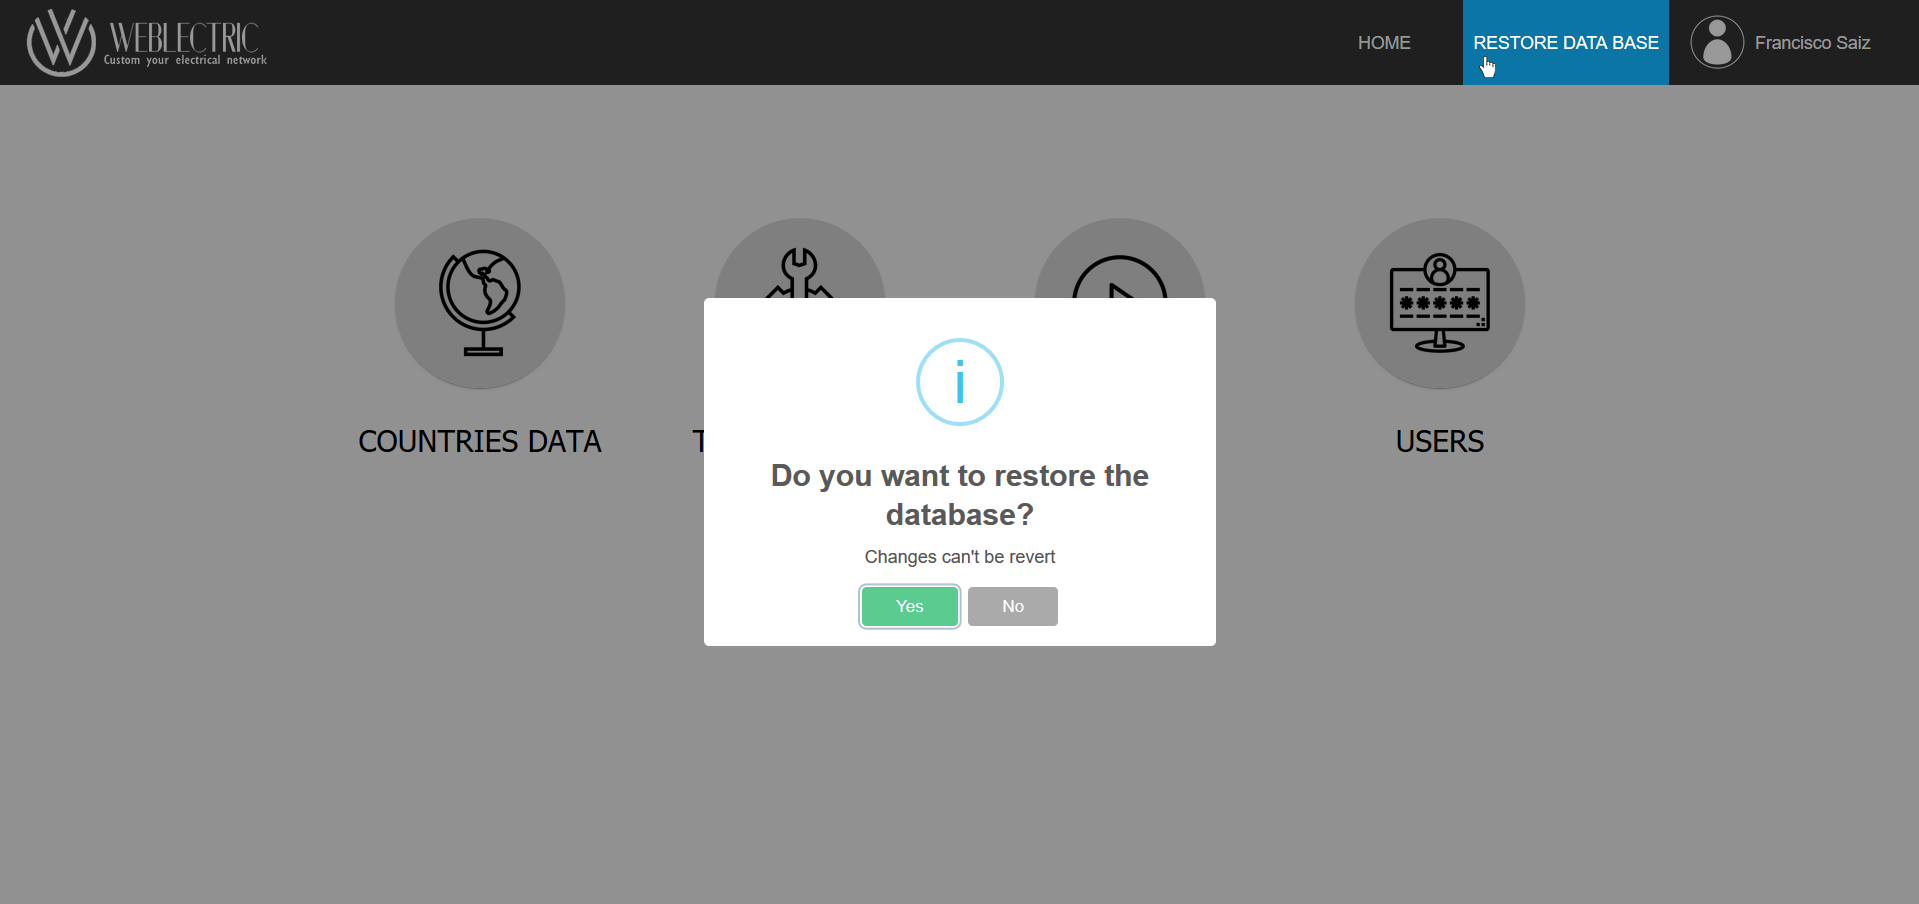
\includegraphics[width=1\textwidth]{/anexos/ManualUsuario/Restore}
	\caption{Mensaje de confirmación previo a la restauración de la base de datos a su estado inicial de test.}	\label{img:Restore}
\end{figure}

\newpage

\subsection{Generación de la simulación}

Desde el \href{https://www.proyectoubu.nesiweb.com/home/home-simulation}{módulo de simulación}, el usuario va a poder preparar la exportación de archivos necesaria para poder ejecutar el algoritmo de optimización.

Como se ve en la figura~\ref{img:SimulationHome}, está la pestaña de \href{https://www.proyectoubu.nesiweb.com/objectives/home}{objetivos} y la pestaña de \href{https://www.proyectoubu.nesiweb.com/simulations/home}{descargas}. Entre los objetivos se distinguen tres grandes grupos, para los que hay diferentes casillas de verificación que al guardarlas como activas, escriben su valor en la sesión actual.
\begin{figure}[h]
	\centering
	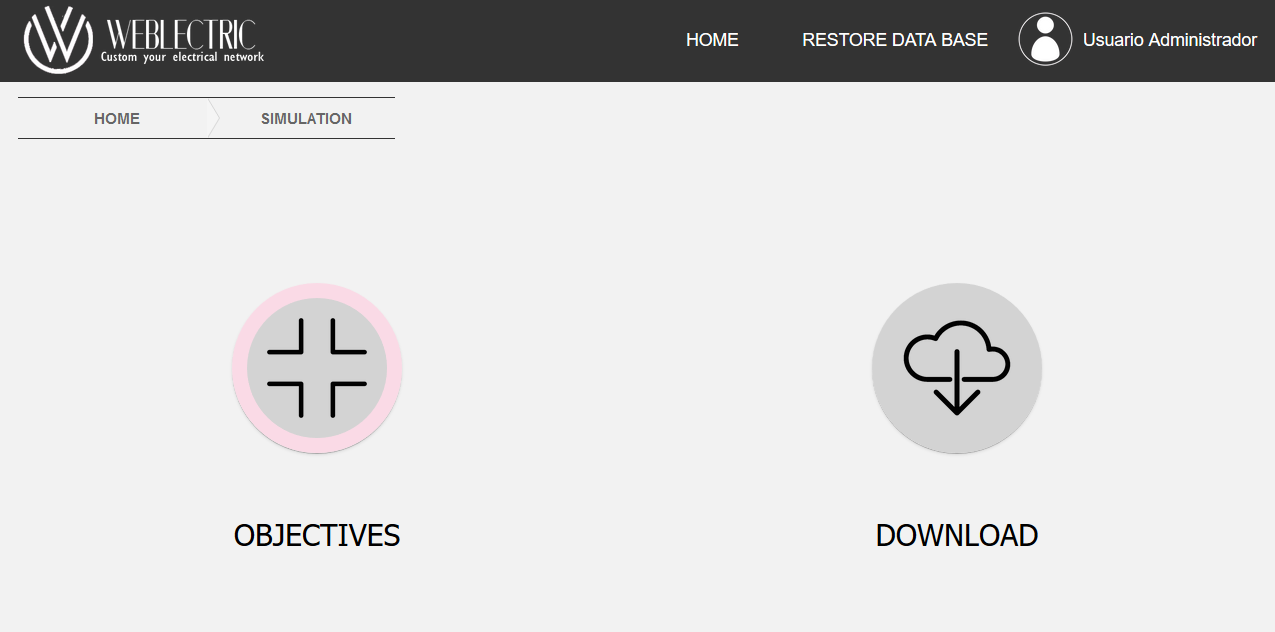
\includegraphics[width=1\textwidth]{/anexos/ManualUsuario/SimulationHome}
	\caption{Pantalla principal del apartado de simulación.}	
	\label{img:SimulationHome}
\end{figure}

Dentro de la pestaña de descargas, aparecen listadas todas las simulaciones que ese usuario ha creado. Desde esta pantalla se pueden realizar tres acciones:
\begin{itemize}
	\item Generar una nueva simulación dándole un nombre. Ver figura~\ref{img:SimulationName}.
	\item Descargar un \textit{.zip} con los archivos necesarios para la simulación.
	\item Eliminar una simulación existente.
\end{itemize}
\begin{figure}[h]
	\centering
	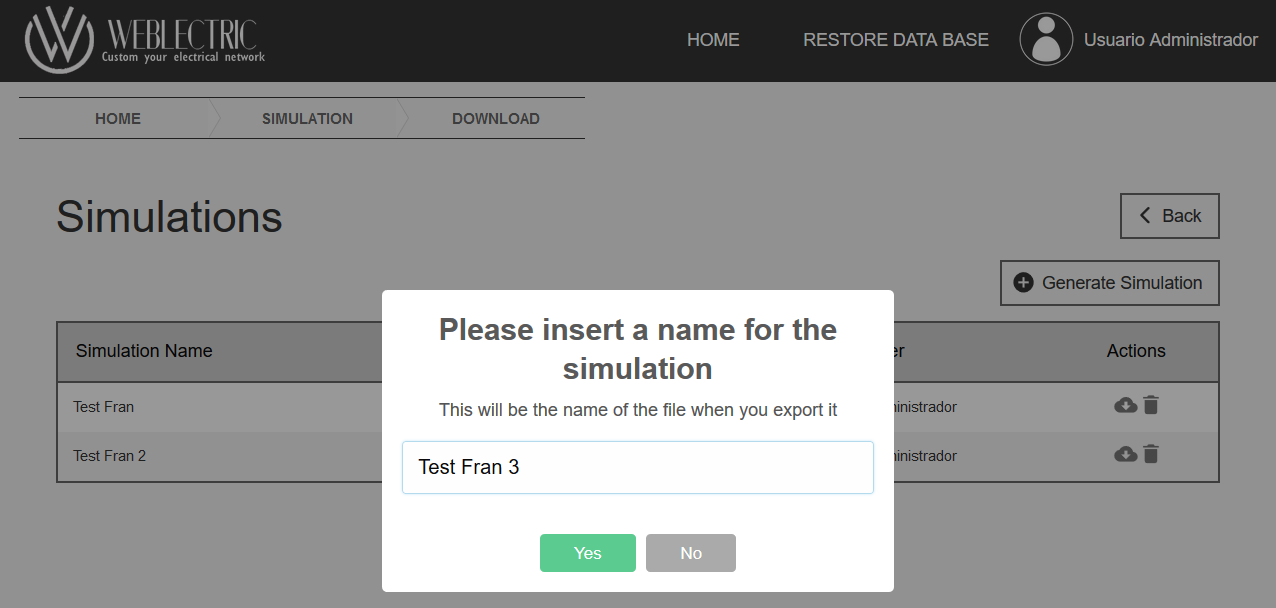
\includegraphics[width=1\textwidth]{/anexos/ManualUsuario/SimulationName}
	\caption{Generar una nueva simulación.}	
	\label{img:SimulationName}
\end{figure}

\newpage

Una vez generada la nueva simulación, se puede descargar el archivo que le corresponde. A continuación, se puede ver la estructura de directorios para el \textit{.zip} descargado. \label{label:export-sim}

\dirtree{%
	.1 /.
	.2 Codigo \desc{Directorio donde se encuentra el algoritmo de optimización del cliente(en \textit{R})}.
	.3 individuo.R \desc{Ejecutable del algoritmo}.
	.2 Data \desc{Directorio donde se encuentran los archivos generados por la aplicación}.
	.3 objectives.json \desc{Archivo en formato \textit{.json} con los objetivos marcados en la aplicación}.
	.3 CapAva.txt .
	.3 Dem.txt .
	.3 ExiCap.txt .
	.3 ExiLin.txt .
	.3 ForMar.txt .
	.3 Fue.txt .
	.3 GenAva.txt .
	.3 Hours.txt .
	.3 Reg.txt .
	.3 Tec.txt .
	.3 Tem.txt .
	.3 TypFue.txt .
	.3 TypLin.txt .
	.3 TypPla.txt .
	.2 Parametros \desc{Directorio donde se encuentran los archivos proporcionados como prueba por el cliente para alimentar el algoritmo de optimización}.
	.3 CapAva.txt .
	.3 Dem.txt .
	.3 ExiCap.txt .
	.3 ExiLin.txt .
	.3 ForMar.txt .
	.3 Fue.txt .
	.3 GenAva.txt .
	.3 Hours.txt .
	.3 Reg.txt .
	.3 Tec.txt .
	.3 Tem.txt .
	.3 TypFue.txt .
	.3 TypLin.txt .
	.3 TypPla.txt .
}

\subsection{Ejecución de la simulación}

Una vez preparada y generada la simulación, para poder ejecutarla es necesario instalar \textit{R} en el equipo. \textit{R} es un entorno y lenguaje de programación con un enfoque al análisis estadístico con el cual, el cliente ha programado el algoritmo.

A continuación, se explicará detalladamente como instalar \textit{R}. Para realizar la instalación es necesario tener privilegios de administrador.

En primer lugar, es necesario descargar \textit{R} para el sistema operativo en uso, en este caso, se instalará la versión 3.5.2 para \textit{Windows}. Está disponible desde el siguiente enlace: 

\url{http://cran.cnr.berkeley.edu/bin/windows/base/R-3.5.2-win.exe}

En segundo lugar, ejecutamos el archivo descargado e instalamos \textit{R} dejando las opciones seleccionadas por defecto.

En tercer lugar, una vez instalado \textit{R}, se ha de descargar \textit{RStudio}, un entorno de desarrollo integrado para el lenguaje de programación R. La descarga se puede realizar desde el siguiente link:

\url{https://download1.rstudio.org/RStudio-1.1.463.exe}

Al igual que en el paso anterior, es aconsejable dejar los valores de configuración por defecto durante la instalación.

En cuarto lugar, habiendo iniciado \textit{RStudio}, se procede a instalar los paquetes, para ello, como se puede observar en la figura~\ref{img:RPackages}, hay que hacer click en el botón ``Install''.

El paquete que hay que instalar se llama ``Rcmdr'' y una vez seleccionado, asegurarse bien de tener marcada la opción de instalar dependencias como bien se representa en la figura~\ref{img:RDependencias}

\begin{figure}[h]
	\centering
	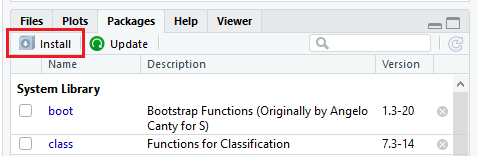
\includegraphics[width=0.9\textwidth]{/anexos/ManualUsuario/RPackages}
	\caption{Instalación de paquetes en RStudio.}	
	\label{img:RPackages}
\end{figure}

\begin{figure}[h]
	\centering
	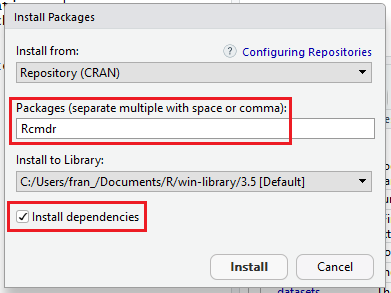
\includegraphics[width=0.6\textwidth]{/anexos/ManualUsuario/RDependencias}
	\caption{Instalación del paquete ``Rcmdr'' y sus dependencias.}	
	\label{img:RDependencias}
\end{figure}

Con todos los componentes necesarios para la ejecución ya instalados, abrimos el archivo \textit{individuo.R} con \textit{Rstudio} y ejecutamos desde el botón ``source'', presente en la figura~\ref{img:RExecute}. Tras unos instantes de ejecución, en la consola de \textit{Rstudio} se puede ver el resultado al igual que en la figura~\ref{img:RSolution}.

\begin{figure}[h]
	\centering
	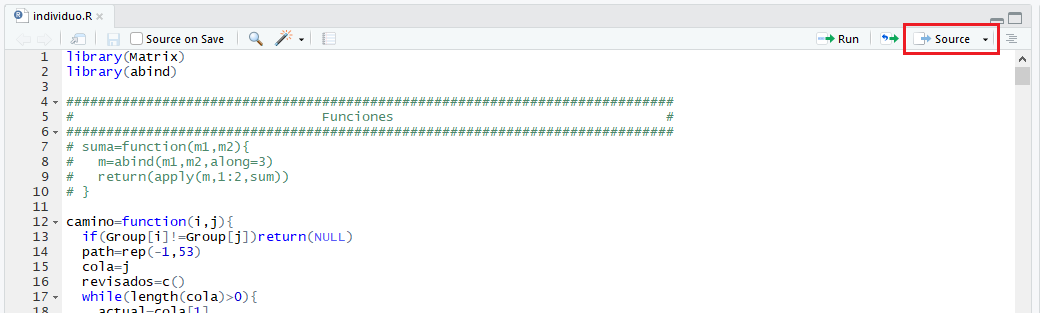
\includegraphics[width=1\textwidth]{/anexos/ManualUsuario/RExecute}
	\caption{Ejemplo de ejecución desde \textit{Rstudio}.}	
	\label{img:RExecute}
\end{figure}

\begin{figure}[h!]
	\centering
	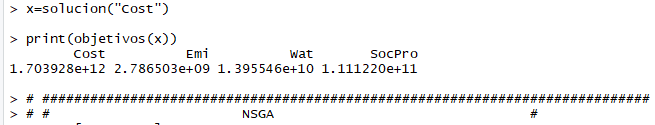
\includegraphics[width=1\textwidth]{/anexos/ManualUsuario/RSolution}
	\caption{Solución tras ejecutar \textit{individuo.R}.}	
	\label{img:RSolution}
\end{figure}

Por último y debido a que el algoritmo funciona únicamente si se cumplen ciertos patrones muy concretos, cabe destacar que en este momento del desarrollo no es posible ejecutar la simulación con los datos extraídos de la web, pues aunque la exportación es correcta y los datos son los deseados, sigue habiendo parámetros fijados por el cliente que no han sido comunicados. 

Además, el desarrollo del apartado de los \href{https://www.proyectoubu.nesiweb.com/objectives/home}{objetivos} no se ha podido finalizar ya que el cliente no ha manifestado especial interés, por tanto, su funcionalidad queda estancada y sin definir. Los objetivos, son datos que en la exportación se han descargado en un formato y estructura no interpretables por el algoritmo.

No obstante, se ha dejado preparada la ejecución para que cuando el cliente mejore la programación del algoritmo evitando los datos estáticos con los que trabaja, la ejecución de la simulación sea posible. Estos datos se almacenan en el directorio \textit{Data}

En la actualidad, la ejecución se lleva a cabo con los datos presentes en el directorio \textit{Parametros}, que como se deja indicado en el apartado donde se explica la exportación de la simulación~\ref{label:export-sim} son datos proporcionados por el cliente, con los cuales la ejecución es satisfactoria.

\newpage


 